%!TEX root = ./thesis.tex

% \chapter{Template}\label{chapter:kapitellabel} %%%%%%%%%%%%%%%%%%%%%%%%%%%%
% \section{Test}
% \subsection{Sub Test}
% Itaque earum rerum hic tenetur a sapiente delectus, ut aut reiciendis voluptatibus maiores alias consequatur aut perferendis doloribus asperiores repellat\cite{aho:dragonbook}. See Table ~\ref{table:speedup1} and ~\ref{table:speedup1} and \ref{figure:helloworld}.

% \begin{table}[!th]
%   \renewcommand{\arraystretch}{1.3}
%   \caption{Speed-Up Table I}\label{table:speedup1}
%   \vspace{4mm} % hack
%   \centering
%     \begin{tabular}{|l||r|r|r|}
%       \hline
%       program            & basline   & algorithm 1  & alogrithm 2\\
%       \hline
%       \hline
%       {\tt simple}       &  30 sec   &  20 sec      &  18 sec     \\
%       \hline
%       {\tt hello world}  &  43 sec   &  27 sec      &  28 sec     \\
%       \hline
%     \end{tabular}
% \end{table}

% \begin{table}[!th]
%   \renewcommand{\arraystretch}{1.3}
%   \caption{Speed-Up Table II}\label{table:speedup2}
%   \vspace{4mm} % hack
%   \centering
%     \begin{tabular}{|l||r|r|r|}
%       \hline
%       program            & basline   & algorithm 1  & alogrithm 2\\
%       \hline
%       \hline
%       {\tt simple}       &  30 sec   &  20 sec      &  18 sec     \\
%       \hline
%       {\tt hello world}  &  43 sec   &  27 sec      &  28 sec     \\
%       \hline
%     \end{tabular}
% \end{table}
% Lorem ipsum dolor sit amet, consectetur adipiscing elit, sed do eiusmod tempor incididunt ut labore et dolore magna aliqua. Ut enim ad minim veniam, quis nostrud exercitation ulla hghgh hhghg mco laboris nisi ut aliquip ex ea commodo consequat. Duis aute irure dolor in reprehenderit in voluptate velit esse cillum dolore eu fugiat nulla pariatur. Excepteur sint occaecat cupidatat non proident, sunt in culpa qui officia deserunt mollit anim id est laborum

% \begin{figure}[!ht]
% \centering
% \sourcecode{main.cpp}
% \caption{Hello World Program}\label{figure:helloworld}
% \end{figure}
% Lorem ipsum dolor sit amet, consectetur adipiscing elit, sed do eiusmod tempor incididunt ut labore et dolore magna aliqua. Ut enim ad minim veniam, quis nostrud exercitation ullamco laboris nisi ut aliquip ex ea commodo consequat. Duis aute irure dolor in reprehenderit in voluptate velit esse cillum dolore eu fugiat nulla pariatur. Excepteur sint occaecat cupidatat non proident, sunt in culpa qui officia deserunt mollit anim id est laborum

% Lorem ipsum dolor sit amet, consectetur adipiscing elit, sed do eiusmod tempor incididunt ut labore et dolore magna aliqua. Ut enim ad minim veniam, quis nostrud exercitation ullamco laboris nisi ut aliquip ex ea commodo consequat. Duis aute irure dolor in reprehenderit in voluptate velit esse cillum dolore eu fugiat nulla pariatur. Excepteur sint occaecat cupidatat non proident, sunt in culpa qui officia deserunt mollit anim id est laborum~\cite{GorillaArm}

% \begin{figure}[!ht] % see https://en.wikibooks.org/wiki/LaTeX/Floats,_Figures_and_Captions for placement parameters
%   \centering
%   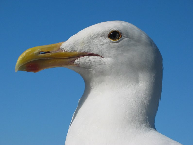
\includegraphics[width=0.5\textwidth]{images/gull.png}
%   \caption{A picture of a gull.}
% \end{figure}

% Lorem ipsum dolor sit amet, consectetur adipiscing elit, sed do eiusmod tempor incididunt ut labore et dolore magna aliqua. Ut enim ad minim veniam, quis nostrud exercitation ullamco laboris nisi ut aliquip ex ea commodo consequat. Duis aute irure dolor in reprehenderit in voluptate velit esse cillum dolore eu fugiat nulla pariatur. Excepteur sint occaecat cupidatat non proident, sunt in culpa qui officia deserunt mollit anim id est laborum

% Lorem ipsum dolor sit amet, consectetur adipiscing elit, sed do eiusmod tempor incididunt ut labore et dolore magna aliqua. Ut enim ad minim veniam, quis nostrud exercitation ullamco laboris nisi ut aliquip ex ea commodo consequat. Duis aute irure dolor in reprehenderit in voluptate velit esse cillum dolore eu fugiat nulla pariatur. Excepteur sint occaecat cupidatat non proident, sunt in culpa qui officia deserunt mollit anim id est laborum

% Lorem ipsum dolor sit amet, consectetur adipiscing elit, sed do eiusmod tempor incididunt ut labore et dolore magna aliqua. Ut enim ad minim veniam, quis nostrud exercitation ullamco laboris nisi ut aliquip ex ea commodo consequat.
% \begin{figure}[H]
%   \centering
%   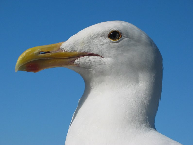
\includegraphics[width=0.5\textwidth]{images/gull.png}
%   \caption{A picture of a gull.}
% \end{figure}
% Duis aute irure dolor in reprehenderit in voluptate velit esse cillum dolore eu fugiat nulla pariatur. Excepteur sint occaecat cupidatat non proident, sunt in culpa qui officia deserunt mollit anim id est laborum

% Lorem ipsum dolor sit amet, consectetur adipiscing elit, sed do eiusmod tempor incididunt ut labore et dolore magna aliqua. Ut enim ad minim veniam, quis nostrud exercitation ullamco laboris nisi ut aliquip ex ea commodo consequat. Duis aute irure dolor in reprehenderit in voluptate velit esse cillum dolore eu fugiat nulla pariatur. Excepteur sint occaecat cupidatat non proident, sunt in culpa qui officia deserunt mollit anim id est laborum

\chapter{Einführung}\label{chapter:kapitellabel}

Zweibeiniges Gehen bietet als Fortbewegungsart durch virtuelle Umgebungen viele Vorteile gegenüber alternativen Fortbewegungsarten.[

    %TODO:Quelle
    ]
beschreibt beispielsweise, ein höheres Präsensgefühl der Nutzer:innen.[
    %TODO: Quelle

]
zeigt dass weniger Motion sickness entsteht wenn sich die Nutzer:innen durch die virtuelle Welt bewegen indem sie gehen.
[
    %TODO: quelle

]
erklärt, dass beim Gehen mehr Sinne stimuliert werden als bei künstlichen Alternativen, wie zum Beispiel der Joystick Steuerung. Tiefensensibilität (Propriozeption) und Gleichgewichtssinn (vestibuläre Wahrnehmung) signalisieren, dass er gerade wirklich geht, während diese Information bei alternativen Fortbewegungsart allein vom visuellen Sinn übermittelt wird.
Leider bring das reale gehen (real walking nach[
    %TODO: quelle

]
) auch den großen Nachteil mit sich, dass es in der Regel auf einen einzelnen Raum (den Trackingspace) beschränkt ist.

Dies entsteht zum einen, durch räumlich limitierte Erfassung (auf Englisch: tracking) der Position und Rotation des Headsets und der Controller bei einigen Technologien (zum Beispiel den Modellen der \textquote{HTC VIVE}-Produktreihe
%TODO:quelle%
), zum anderen durch die Raumgröße der meisten VR-Setups.

Zwar gibt es dazu auch Ausnahmen, ( siehe z.B.[
    %TODO: quelle microsoft studie
]
), jedoch sind diese dann mit großem Aufwand verbunden und nicht für jede Endnutzer:in umzusetzen.

\section{Redirections Techniques} %oder lieber deutsch???
%sind impossible spaces überhaupt redirected walking?
Eine Herangehensweise dieses Problem zu Umgehen sind so genannte \textquote{Redirection Techniques} (besser bekannt als Redirected Walking, diese Begriffe werden oft austauschbar verwendet (nach [
    %quelle steinicke übersicht paper

])). Dies ist ein Sammelbegriff für Techniken bei denen die Nutzer:in mit Manipulationen der Fortbewegungsart durch den Trackingspace navigiert wird.
%  Dabei wird die Illusion aufrecht erhalten sie würde sich unverändert, frei bewegen.
So lässt sich die Nutzer:in von den äußeren Begrenzungen des Trackingspaces fern halten, und die virtuell begehbare Fläche vergrößern.
Im folgenden werde ich nun zwei dieser Techniken genauer vorstellen.

\subsection{Rotationgains}
%TODO: quelle steinicke zusammenfassung der techniken
Rotationgains werden Kopfrotationen hinzugefügt sodass sich die virtuelle Kamera leicht schneller oder langsamer dreht als der reale
Kopf mit dem VR-Headset. Kopfrotationen lassen sich mit der Schreibweise
$$ R_{real} := (pitch_{real}, yaw_{real}, roll_{real}) $$
darstellen, wobei pitch, yaw und roll
die Eulerschen Winkel der Kopfrotation darstellen. Der Rotationgain wird dann als Quotient des virtuellen Winkels und des realen Winkels definiert also:
$$ gR := \frac{R_{virtual}}{R_{real}} $$
Für alle 3 Winkel kann ein Rotationgain angewandt werden.
Dieses Anwenden funktioniert indem der Rotationgain $gR$ mit dem Winkel der realen Kopfrotation $\alpha$ multipliziert wird also:
$$ gR * \alpha $$
Da für jeden Winkel der Kopfrotation ein Rotationgain definiert werden kann werden Rotation gains folgendermaßen dargestellt:
$$(gR_{pitch}, gR_{yaw}, gR_{roll})$$
%TODO: inline?
In der Regel wird für Redirection ein Rotationgain auf den $yaw_{real}$ Winkel der Kopfrotation angewandt.
[
    %quelle steinicke techniken
]
Durch anwenden eines rotation gains kann der virtuelle Trackingspace um den realen Trackingspace mit dem Drehpunkt der Nutzerposition herum rotiert werden.
Für den Nutzer kann so die Illusion entstehen er würde über die Grenzen des Trackingspaces hinaus schreiten können, ohne dies zu tun. (Siehe grafik)
%TODO: grafik.

\subsection{Impossible Spaces}
Um den begehbaren Bereich eines Trackingspace noch weiter zu vergrößern haben sich Suma et al. \cite{impossible-spaces-suma} eine Technik ausgedacht bei der zwei oder mehr Räume in überlappenden Flächen liegen, allerdings nur einer zur Zeit angezeigt wird. Es gibt dann unterschiedliche Bedingungen, wann welcher der Räume angezeigt wird. Beispiels weise wird Raum $A$ nur angezeigt wenn die Nutzer:in den überlappenden Raum durch Tür $a$ betritt und Raum $b$, wenn sie ihn durch Tür $b$ betritt.
%TODO: grafik?
Dafür ist es also notwendig $x$ verschiedene states
%TODO: übersetzung
zu setzen sodass immer einer $x$ verschiedener Räume angezeigt wird. Des weiteren ist es Notwendig einen Bereich zu erschaffen in dem zwischen den states gewechselt werden kann, ohne dass die Nutzer:in es merkt.

\section{Generierte Level} %prozedural, oder zufällig? oder pseudozufällig?

Klassischer weise werden Level in Computerspielen und virtuellen Umgebungen von Leveldesignern designed. Dies erfordert Zeit und know-how. %TODO: formulierung
Der Arbeitsaufwand wächst (linear) mit der Größe des Levels, deshalb ist es unmöglich endlos große Level zu erschaffen. Eine alternative Levelerstellungsweise ist das so genannte \textquote{Prozedurale Generieren}(Auch \textquote{Prozedurale Synthese} genannt. Dabei wird das Level von einem Algorithmus erschaffen, und kann somit endlos große Welten erschaffen.
%verschiedene Arten von prozeduraler generiung und dazu beispiel wie minecraft, rogue etc. mit quellen.

In dem hier vorgestellten Experiment


\chapter{Verwandte Arbeiten}\label{chapter:kapitellabel}

In diesem Kapitel werden wissenschaftliche Arbeiten vorgestellt mit denen diese Arbeit zusammenhängt. Dabei werde ich zunächst auf solche Arbeiten eingehen, die sich mit dem Thema Real-Walking in virtuellen Umgebungen beschäftigen, danach verschiedene redirection Techniken vorstellen und dann auf das Thema der Level-Generierung eingehen. Zunächst stelle ich generelle Arbeiten zu dem Thema Real-Walking und dann zu Redirection Techniken vor, danach gehe ich konkreter auf die in dieser Studie sehr im Fokus liegenden Rotationgains ein um danach die auch in dieser Studie genutzten Impossible Spaces vorzustellen. Als nächstes stelle ich dem Leser noch Arbeiten vor die sich damit beschäftigt haben Level auf eine automatische Art und Weise zu generieren. Dabei werde ich mich sowohl mit Artikeln über die genauen Definition dieses Bereichs beschäftigen, als auch eine Taxonomie zur Einordnung von Prozeduren zur Inhaltsgenerierung zitieren. Die Kombination von generierten Leveln und Redirection-Techniken führen zu dem sogenannten \textquote{Infinite-Walking}. Mit den Arbeiten zu diesem Thema wird das Kapitel abgeschlossen.

\section{Real-Walking}
1995 zeigen Slater et al. \cite{taking-steps}, dass Proband:innen eine höheres Präsensgefühl zeigten wenn sie die von ihm vorgestellte Technik \textquote{Walking-In-Place} nutzen als wenn sie per Knopfdruck durch die Welt bewegten. Hierbei handelte es sich um eine virtual-walking Technik bei der die Proband:innen ein eine Gehbewegung simulierten die dann digital erfasst und in Virtuell Fortbewegung umgewandelt wurde. Dieses Experiment wurde 1999 von Usoh et al. \cite{usoh-vergleich-1999} repliziert, wobei nun die Option wirklich zu gehen (\textquote{Real-Walking}) gegeben war. Dabei hatten die Proband:innen nochmal ein signifikant höheres Präsensgefühl, als bei den beiden anderen Optionen (Virtual-Walking und Push-Button-Fly).
Des weiteren zeigen Arbeiten wie \cite{benefits-real-walking} und \cite{locomotion-path-integration}, dass virtuelle Fortbewegungsarten, die anders als real-walking nicht den vestibulären Sinn und die Propriozeption stimulieren, wahrscheinlicher die sogenannte \textquote{Simulator-Sickness} auslösen und, dass die User:innen damit weniger effektiv navigieren.

Wenn Designer eine Real-Walking-Umgebung erstellen müssen sie dabei schon die Dimensionen des Trackingspaces kennen. Da man aber nicht davon ausgehen kann, dass unterschiedliche Nutzer:innen gleiche Trackingspacedimensionen zur Verfügung haben entsteht ein Problem, dass Marwecki et al. in ihrer Arbeit \cite{scenograph} zu Lösen versuchen. Sie stellen dabei das Softwaresystem \textquote{Scenograph} vor, welches große virtuelle Umgebungen in mehrere kleinere, teilweise anders geformte, Umgebungen, mit prozedural generierten Verbindungen, aufteilt ohne dabei die narrative Struktur der Ursprünglichen Umgebung zu verändern.

Allerdings gibt es auch andere Ansätze um Nutzer:innen mit begrenztem Trackingspaceplatz Real-Walking-Erfahrungen zu ermöglichen, wie beispielsweise den virtuellen Bereich, der von der Nutzer:in begehbar ist, zu vergrößern.
Eine vielversprechende Art dies zu erreichen sind Redirection-Techniken.

\section{Redirection Techniken}
Razzaque et al. \cite{rdw-razzaque} stellten 2001 die Technik des \textquote{Redirected-Walking} vor, bei der die Nutzer:innen unwissentlich durch den Trackingspace gelenkt werden, dabei aber die Illusion entsteht, sie würden sich über die Grenzen dessen hinausbewegen. Die Technik basiert darauf, dass der visuelle Sinn dominanter ist als andere Sinne, mit denen man seine Orientierung im Raum bestimmen kann \cite{conflicting}. Seit dem gibt es zahlreiche weitere Techniken um den selben Effekt zu erzielen oder um ihn weiterzuentwickeln. Der Ansatz die verschiedenen Manipulationseffekte als \textquote{Gains} zu beschreiben findet sich bei Steinicke et al. \cite{detection-thresholds}. Dort wird untersucht wie subtil diese Manipulationen sein müssen um nicht von der Nutzer:in erkannt zu werden.

Es konnte gezeigt werden, dass Proband:innen in virtuellen Umgebungen, die Redirection-Techniken nutzen um Real-Walking zu ermöglichen, signifikant besser unbewusst räumliches Wissen über diese Umgebungen sammelten, signifikant bessere Navigation und Wegfindung aufwiesen und die Größe der Umgebung signifikant besser einschätzen konnten als in Umgebungen, die andere Fortbewegungsarten nutzen, wie Walking-In-Place, Joystick-Steuerung oder Teleportation \cite{peck-vergleich-2011}, \cite{langbehn-vergleich-2018}.

Eine Taxonomie über die verschiedenen Redirection Techniken stellten 2012 Suma et al. \cite{taxonomy} vor. Die unterschiedlichen Techniken werden in die Kategorien: \textquote{Repositioning} (Repositionierung) oder \textquote{Reorientation} (Reorientierung), \textquote{Subtle} (subtil) oder \textquote{Overt} (unverborgen), und \textquote{Discrete} (diskret) oder \textquote{Continuous} (kontinuierlich) unterteilt.

%curvature games paper?

\subsection{Rotation Gains}

Bei Rotationgains handelt es such nach Sumas Taxonomie \cite{taxonomy} um eine kontinuierliche, subtile Reorientierungstechnik. In der Arbeit \cite{detection-thresholds} untersuchten Steinicke et al. verschiedene subtile Redirection-Techniken darauf, wie stark die Manipulation sein darf, bevor Proband:innen erkennen ob sie eingesetzt wurde oder nicht. Dazu teilt er die verschiedenen Elemente, die für Redirected Walking eingesetzt werden, in drei verschiedene Gains ein: \textquote{Translation-Gains}, \textquote{Rotation-Gains} und \textquote{Curvature-Gains}. Es stellte sich heraus, dass Nutzer:innen physisch um bis zu 49\% mehr oder um bis zu 20\% weniger als die wahrgenommene virtuelle Rotation, rotiert werden können, ohne die Diskrepanz zu bemerken.

Des weiteren wurde festgestellt, dass Distanzen unbemerkt um bis zu 14\% herunter- oder um bis zu 26\% heraufskaliert werden können und, dass Nutzer:innen erst bemerken, dass Sie in einem Kreisförmigem Bogen durch den Trackingspace geleitet werden, wenn dessen Radius 22m oder kleiner ist.
%formulierung sehr nah an abstract, direct quote?, umformulieren?

\subsection{Impossible-Spaces}

Bei \textquote{Impossible-Spaces} handelt es sich um eine von
Suma et al. \cite{impossible-spaces-suma} vorgestellte Redirection-Technik, bei der sich die Architektur der virtuellen Umgebung auf nicht-euklidische Weise verändert, sodass solche Gebiete in der Realität nicht existieren könnten.
Die Räume überlappen einander, allerdings wird jeweils nur einer der überlappenden Räume angezeigt. Hierbei handelt es sich nach der schon erwähnten Taxonomie um eine subtile diskrete Redirection-Technik.

In einer Forschungsdemonstration \cite{redirected-spaces} stellten Langbehn et al. eine Weise vor mit der Impossible-Spaces mit traditionelleren Redirected-Walking Methoden (in diesem Fall Curvature-Gains)
%TODO: sind bending und curvature gains das selbe?
kombiniert werden können, sodass beide Methoden ihren Effekt beitragen können.

\section{Prozedural generierte Level}

\subsection{Definition}

Der Artikel \cite{sbpcg} von Togelius et al. definiert prozedurale Generierung von Spiel-Inhalten (procedural (game-)content generation oder auch PCG) als:

\begin{quotation}
    \textquote{[...] creating game content automatically, through algorithmic means.}
\end{quotation}

\begin{quotation}
    (\textquote{[...] algorithmisch, automatisch, (Computer-)spiel Inhalte erstellen.})
\end{quotation}

In ihrer späteren Arbeit hingegen \cite{what-is-pcg} definieren Togelius et al. PCG folgendermaßen neu:
\begin{quotation}
    \textquote{We can therefore tentatively redefine PCG as the algorithmical creation of game content with limited or indirect user input.}
\end{quotation}

\begin{quotation}
    (\textquote{Wir können PCG daher versuchsweise als die algorithmische Erstellung von Spielinhalten mit begrenzter oder indirekter Benutzereingabe neu definieren.})
\end{quotation}


um unter anderem miteinzubeziehen, dass einige PCG-Algorithmen Nutzer- oder Designerinput miteinbeziehen können und somit nicht mehr \textquote{automatisch} Inhalte generieren. Ausserdem wollen sie in der Definition festhalten, dass Nutzerinput typischerweise zumindest indirekt (beispielsweise durch Druck eines Startknopfes) erforderlich ist um Inhalte zu generieren.

Mit (Spiel-)Inhalten sind in diesen Definitionen unterschiedlichste Elemente in Videospielen gemeint. Unter anderem Texturen, Musik oder auch die Geschichte des Spiels können prozedural generiert werden. Im Rahmen dieser Arbeit hingegen beschäftige ich mich lediglich mit PCG zur Erstellung von Leveln.

\subsection{Taxonomie}

In ihrer Arbeit \cite{sbpcg} stellten Togelius et al. eine Taxonomie für PCG vor, die aus folgenden Kategorien besteht:

\textquote{Online versus offline} (Zur Laufzeit versus während der Entwicklung),

\textquote{Necessary vs optional} (Müssen die Spieler:innen den generierten Bereich des Spiels absolvieren oder nicht?),

\textquote{Random seeds versus Parameter Vectors} (auch: \textquote{degrees of control}: Wieviel Einfluss hat die Spieler:in auf den Generierten Inhalt, wird nur ein zufälliger RNG-Seed (Random-Number-Generator-Seed) als Eingabe in den Zufallsgenerator genutzt oder wird sein bisheriges Spielverhalten analysiert und bei der Generierung beachtet?),

% \textquote{Generic vs adaptive} () irgendwie nur im pcg buch und nicht im paper,

\textquote{Stochastic vs deterministic} (Wird bei gleicher Eingabe (abgesehen vom RNG-Seed) auch der gleiche Inhalt generiert?) und

\textquote{Constructive vs generate-and-test} (Generiert der Algorthmus direkt nur korrekte Ausgaben, oder funktioniert er so, dass er fortlaufend Versuche generiert und dann validiert ob sie korrekt sind und sie dann erst ausgibt.) %und

% \textquote{Automatic generation vs mixed authorship}.

Der in dieser Arbeit beschriebene PCG-Algorithmus lässt sich dementsprechend eher in diese Kategorien Taxonomie einordnen, als in ihre jeweiligen Alternativen: Online, necessary, random seeds,
 %generic,
 stochastic and constructive. % and automatic.
%TODO: übersetzen

\section{Infinite walking}
Viele der redirection Techniken ermöglichen das (erlebte) hinaustreten über den Rand des Trackingspaces, doch dennoch bleibt die begehbare Fläche limitiert. Solange die virtuelle Umgebung von menschlichen Designern erschaffen werden muss ist sie begrenzt. Wenn jedoch PCG genutzt wird um die virtuelle Umgebung zu erschaffen lässt sie sich theoretisch endlos weit durchschreiten, weil die Generierung während dem Erkunden der Welt fortgeführt werden kann.
Wenn die virtuelle Umgebung also, mit Hilfe von PCG, theoretisch endlos weit erkundet werden kann spricht man vom \textquote{Infinite-(Real)-Walking}.
In der Regel lässt sich dieser Zustand %?
erreichen indem man Redirection-Techniken (um über den Trackingspace hinaus gehen zu können) mit prozeduraler Levelgenerierung (um die Welt weiter zu während der Laufzeit weiter zu generieren) kombiniert.

Ein Beispiel für eine solche Technik stellen Vasylevska et al. in ihrer Arbeit \cite{flexible-spaces} vor. Ihr Algorithmus generiert fortlaufend Räume, innerhalb des Trackingspaces, die einander überlappen können (Impossible-Spaces) und verbindet sie mit Korridoren, sodass die Nutzer:in von einem Raum zum nächsten gehen kann. Praktisch ist diese Technik besonders bei Umgebungen in denen der Inhalt der Räume mehr im Fokus steht als das spezifische Layout der Räume wie beispielsweise einem Museum.

Einen sehr ähnlichen Ansatz nutzt das VR-Spiel \textquote{Tea for God} \cite{tea-for-god} bei dem die Nutzer:in durch ein endlos scheinendes Labyrinth von Korridoren gehen kann. Der Entwickler Jarosław (Void Room) Ciupiński erklärt in seinen Devlogs (beispielsweise \cite{tea-for-god-devlog-a} oder \cite{tea-for-god-devlog-b}) genauer wie der Ansatz funktioniert.
Die Welt besteht aus einem prozedural generierten Netz von verbundenen Zellen, die jeweils einen Raum repräsentieren und mit Korridoren verbunden sind. Auch hier basieren die Räume auf den vorher erwähnten Impossible Spaces.
%In seinem devlog \cite{tea-for-god-devlog-b} erwähnt der Autor die eben erwähnte Arbeit von Vasylevska et al. \cite{flexible-spaces}, was darauf hindeuten könnte, das Spiel wäre von dem Ansatz der flexible spaces inspiriert.

Einen anderen Ansatz verfolgt das in der Arbeit \cite{microsoft} von Cheng et al. vorgestellte Projekt \textquote{VRoamer}.
Hier erkundet die Nutzer:in eine On-The-Fly generierte virtuelle Umgebung (auch hier besteht diese aus Räumen und Korridoren), während er durch die reale Welt läuft. Die Generierungssoftware erhält einen 3D-Kamera Input und kann so Wände, Säulen, Gegenstände, andere Menschen etc. beachten und dementsprechend die virtuelle Welt anpassen. Dort wird dann ein virtueller Gegenstand platziert, sodass die Nutzer:in nicht mit den Hindernissen der realen Welt kollidiert.
Diese Technik ist nur bei VR-System anwendbar, die nicht auf einen Trackingspace beschränkt sind, sondern (zum Beispiel mit Kameras am HMD (Head-Mounted-Display)) ihre Umgebung, und somit auch ihre eigene Position und Orientierung benötigen. Die Möglichkeit die virtuelle Umgebung zu erkunden sind hier also nur durch den realen Platz, den die Nutzer:in zur freien Begehung zur Verfügung hat limitiert. Streng genommen gilt die Definition von Infinite-Walking hier also nicht, sie sollte an dieser Stelle aber dennoch Erwähnung finden.

\section{Einordung dieser Arbeit}
Ähnlich zu der Arbeit \cite{flexible-spaces} werde ich in dieser Arbeit eine Methode vorstellen, wie mit verschiedenen Redirection-Techniken und einem PCG-Algorithmus eine virtuelle Umgebung mit Infinite-Walking erstellt werden kann.
Vergleichbar mit den Arbeiten \cite{peck-vergleich-2011} und \cite{langbehn-vergleich-2018} werde ich diese Methode dann in einem Experiment unter Testbedingungen mit alternativen Fortbewegungsarten, die dementsprechend kein Real-Walking ermöglichen auf verschiedene Faktoren vergleichen.
%schon genug? was soll da schon noch hin?

\chapter{Implementierung}\label{chapter:kapitellabel}

In diesem Kapitel werde ich die technische Umsetzung für das in dieser Arbeit vorgestellte Experiment vorstellen. Dabei werde ich im Detail erklären, wie die unterschiedlichen Module des Quelltext funktionieren und dementsprechend offen legen, wie eine solche Infinite-Walking Umgebung implementiert werden kann. Die gesamte Programmierung für dieses Projekt ist in der Entwicklungsumgebung Unity (Version:) \cite{unity} und dementsprechend mit der Programmiersprache \textquote{C\#} erfolgt. Um die Software während der Entwicklung testen zu können und um damit das Experiment durchführen zu können wurde mir freundlicherweise eine \textquote{Oculus Quest 2} \cite{quest} Datenbrille, vom Arbeitsbereich Mensch-Computer-Interaktion der Universität Hamburg zur Verfügung gestellt. Um mit der Schnittstelle davon zu interagieren nutzt das Projekt das, von Oculus frei zur Nutzung gestellte, \textquote{Oculus Integration SDK} für Unity \cite{integration}.
%Space extender erwähnen

\section{Scripts}
Um die Implementierung vorzustellen wird an dieser Stelle zuerst ein UML-Klassendiagramm vorgestellt, indem die Relationen zwischen den verschiedenen Klassen ersichtlich sind, um danach in einzelnen Absätzen nochmal genauer auf die verschiedenen Klassen, ihre Funktionsweise und ihren Zweck einzugehen.

\subsection{Klassendiagramm}
Um das Diagramm übersichtlich zu halten beschränkt es sich
%TODO: fast?
ausschließlich auf die Relationen zwischen den Klassen, es wird also nicht wie sonst in UML-Klassendiagrammen üblich die gesamte Schnittstelle aller Klassen inklusive ihren Attributen und ihren Methoden aufgelistet.
%TODO: ausser für sehr zentrale?
Aus dem selben Grund wurden auch Grundklassen/-typen mit denen Standardmäßig in Unity gearbeitet wird (zum Beispiel \textquote{Vector3}, \textquote{MonoBehaviour} oder \textquote{GameObject}) weggelassen.

\begin{center}
    \begin{tikzpicture}
        \begin{umlpackage}{Assets/Scripts}

        \umlemptyclass[x=4,y=1]{GenerateLevel}

        \umlclass[x=10,y=-1]{GeneratorOculusInterface}{}{
        }
        \umlclass[x=7,y=-5]{RoomGenerator}{}{
        }
        \umlclass[x=4,y=-1]{RoomAndProgressManager}{}{
        }

        \umlclass[x=2,y=-5]{RotationGainMechanism}{}{
        }

        \umlclass[x=10.8,y=-8]{RotationRedirectorCollision}{}{
        }

        \umlclass[x=4,y=-7]{SceneLoader}{}{
        }

        \umlinterface[x=5,y=-9.5]{INumberPadListener}{}{
        }

        \umlclass[x=2,y=-12]{NumberPadScript}{}{
        }

        \umlclass[x=8,y=-12]{NumberPadButton}{}{
        }

        \end{umlpackage}

        \begin{umlpackage}[x=10,y=5]{SpaceExtender}
        \umlclass{RotationRedirector}{}{}
        \end{umlpackage}

        \begin{umlpackage}[x=2,y=5]{Oculus Integration SDK}
        \umlclass{OVRManager}{}{}
        \end{umlpackage}

        \umldep[geometry=-|, anchors= 5 and -90, align2=left]{GenerateLevel}{RotationRedirector}

        \umldep[geometry=-|, anchors= 0 and 85, align2=left]{GenerateLevel}{RoomGenerator}

        \umldep[geometry=-|, anchors= -5 and 90, align2=left]{GenerateLevel}{RotationRedirectorCollision}

        \umldep[geometry=|-|, weight=0.7, anchors= 160 and -90, align2=left]{GeneratorOculusInterface}{OVRManager}

        \umlinherit[geometry=|-, anchors= 160 and 180]{RotationGainMechanism}{INumberPadListener}

        \umlinherit[geometry=-|, anchors= 180 and 90]{SceneLoader}{INumberPadListener}

        \umluniassoc[geometry=-|-, anchors= 180 and 0]{NumberPadButton}{NumberPadScript}

        \umluniassoc[geometry=|-|, anchors= 90 and -90]{NumberPadScript}{INumberPadListener}

        \umluniassoc[geometry=-|, anchors= 180 and -90]{RotationRedirectorCollision}{RotationGainMechanism}

        \umluniassoc[geometry=|-|, anchors= 110 and -90]{RotationGainMechanism}{RoomAndProgressManager}

        \umluniassoc[geometry=|-|, anchors= -50 and 95]{RoomAndProgressManager}{RoomGenerator}

        \umluniassoc[geometry=|-|, anchors= -90 and 90]{GenerateLevel}{RoomAndProgressManager}

        \umluniassoc[geometry=|-, anchors= 120 and -15]{GeneratorOculusInterface}{GenerateLevel}

        \umluniassoc[geometry=|-|, anchors= 150 and -145, align2=left]{RotationGainMechanism}{RotationRedirector}

        \umluniassoc[geometry=-|, anchors= 180 and 145, align2=left]{SceneLoader}{NumberPadScript}

        \end{tikzpicture}
        \vspace{4cm}
\end{center}

\subsection{Vorstellung der Klassen}
\begin{multicols*}{2}
    \paragraph{GeneratorOculusInterface}
    Kommuniziert mit der Schnittstelle des \textquote{Oculus Integration SDK} um Informationen die im Projekt benötigt werden bereitzustellen. Die wichtigsten Informationen die hier geliefert werden sind die Koordinaten der Begrenzungsecken des Trackingspaces. Die Nutzer:in der Oculus Quest 2 stellt im Setup der Brille den sogenannten \textquote{Guardian} ein. Dies ist dann eine Begrenzung die sie um den begehbaren Raum in dem sie sich befindet zieht und der immer dann in der virtuellen Realität eingeblendet wird, wenn sie dieser Begrenzung mit den Hand-Controllern oder der Datenbrille zu nahe kommt. Diese Begrenzung ist allerdings nicht rechteckig, was für den hier vorgestellten Levelgenerierungsalgorithmus aber notwendig wäre. Doch das Oculus SDK bietet in seiner Schnittstelle an, das größte, in diese Begrenzung passende, Rechteck auszugeben, dies ist dann die Grundlage für die Raumgenerierung. Zudem ist diese Klasse dafür zuständig, je nach ausgewählter Testbedingung entsprechende Einstellungen an das Oculus SDK zu übergeben.
    %Zum Beispiel ist bei der Real-Walking Bedingung erforderlich den \textquote{Tracking Origin Type} der Erfassung auf \textquote{Stage} zu setzen, sodass

    \paragraph{RoomGenerator}
    Implementiert die Generierung der einzelnen Räume. Dafür liegt in dieser Klasse die zentrale \textquote{Generate}-Methode. Anhand von den vier Eckkoordinaten des Raumes, der Richtung in die der Raum zeigen soll und verschiedener Zusatzeigenschaften wie zum Beispiel, der Tiefe des zu generierenden Korridors, der Höhe der zu generierenden Türen, der Dicke der Wände und der Höhe des zu generierenden Korridors erzeugt diese Methode das GameObject für den zu generierenden Raum, erzeugt das entsprechende Mesh für den Korridor und platziert die ansonsten nötigen Objekte (zum Beispiel Türen, Tafel, Eingabefeld) an den richtigen Positionen. Um die Tür nicht immer mittig zu platzieren bekommt die \textquote{Generate}-Methode ausserdem einen Zufallswert zwischen 0 und 1 übergeben. Dieser bestimmt dann die Position der Tür, die in den Korridor hineinführt. (0 bedeutet ganz links, 1 hingegen ganz rechts).
    Des weiteren bietet diese Klasse mehrere Methoden an, die Berechnungen über den Raum, den sie generiert haben anstellen können. So kann man sich beispielsweise berechnen lassen ob der Korridor des Raumes auf der längeren, oder der kürzeren Kante des Grundrechtecks liegt, wie die Koordinaten des Mittelpunkts des ganzen Raumes sind und wie die Koordinaten des Mittelpunktes des Bereichs vor dem Korridor sind. (An diese Stelle im ersten Raum wird die Proband:in bei den Testbedingungen, in denen kein real-walking stattfindet, teleportiert.) Die Klasse besteht aus circa 1000 Zeilen Programmierung und ist somit die längste selbst geschriebene Klasse des Projektes.

    \paragraph{GenerateLevel}
    Diese Klasse implementiert den prozeduralen Levelgenerierungsalgorithmus der genauer in
    %Todo: kapitel finden
    beschrieben wird. Sie ist die zentrale Klasse des Projektes. In ihren öffentlichen Attributen können die Einstellungen für die zu generierende Testbedingung verändert werden. In ihrer \textquote{Generate}-Methode implementiert sie den Levelgenerierungsalgorithmus und verbindet darin die restlichen Teilmodule des Projekts. Sie ist also nicht nur dafür verantwortlich die \textquote{Generate}-Methode der \textquote{RoomGenerator}-Klasse mit den richtigen Eingabewerten aufzurufen, sondern platziert auch die Rotation-Gain Funktionalität an die richtige Stelle, und übergibt die Generierten Räume an den \textquote{RoomAndProgressManager}, in dem sie in einer Liste gespeichert werden.

    \paragraph{RoomAndProgressManager}
    Ist dafür zuständig den Fortschritt der Proband:in zu verfolgen und entsprechend zu reagieren wenn es notwendig ist. Beispielsweise öffnet er die entsprechenden Türen, wenn ein Raum abgeschlossen ist.
    Des weiteren hält diese Klasse Instanzen der GameObjects für die Räume, in einer Liste, sodass sie dazu in der Lage ist an den zugehörigen RoomGenerator-Instanzen Methoden aufzurufen. Um später vergleichen zu können wie gut die Einschätzung der Proband:innen war misst diese Klasse ausserdem die von der Proband:in fortbewegte Strecke. Wenn der letzte Raum des aktuellen Versuchs erreicht wurde übergibt sie die entsprechenden Daten an den FirebaseHandler der diese dann an eine Cloud-Datenbank verschickt sodass der Versuchsdurchgang im Nachhinein ausgewertet werden kann.


    \paragraph{RotationGainMechanism}
    Diese Klasse implementiert den Mechanismus, der in der Real-Walking Bedingung bei den jeweiligen Räumen angewandt wird um den genauen Ablauf des RotationGains zu bestimmen. Er zeigt die Zahlen auf der Tafel an, verwertet die Eingabe des Eingabefelds, startet den Rotation-Gain und beendet ihn auch wieder. Er signalisiert dem RoomAndProgressManager wenn der Rotation-Gain vollständig ist, also sich der Trackingspace also um 90\textdegree\ gedreht hat, und die Proband:in dann eine richtige Eingabe tätigt, dass der Raum abgeschlossen ist, sodass sich die Tür öffnet. In den anderen Bedingungen ist er dafür verantwortlich dies nach einer zufälligen, geringen, Anzahl richtiger Eingaben in das NumberPad zu tun, sodass die Proband:in auch in diesen Bedingungen den selben Ablauf erleben.

    \paragraph{SceneLoader}
    Bei betreten des Levels sieht die Proband:in ein virtuelles Eingabefeld, in dass sie die verschiedenen Testbedingungen (A1-C3, siehe Kapitel
    % TODO: kapitel nennen
    ) eingeben kann um den Versuch zu starten. Der SceneLoader ist dafür zuständig auf diese Eingabe entsprechend zu reagieren und die entsprechende Bedingung zu Laden. Dazu verändert der die Attribute der \textquote{GenerateLevel}-Instanz und ruft dann auf ihre die \textquote{Generate}-Methode auf.

    \paragraph{RotationRedirectorCollision}
    Kleine Hilfsklasse, die erkennt ob der Nutzer sich gerade in dem entsprechenden Bereich befindet, indem der Rotation-Gain aktiv sein soll.

    \paragraph{Door}
    Die Türen nutzen dieses Script. Auf ihm kann die Methode \textquote{OpenDoor} aufrufen um sie zu öffnen.

    \paragraph{Dissolvable}
    Wird von der \textquote{Door}-Klasse genutzt um der Tür die Funktionalität zu geben fließend zu verschwinden. Dafür nutzt sie einen entsprechenden Shader.

    \paragraph{INumberPadListener}
    Die Klassen die über Eingaben in einem NumberPad informiert werden wollen können dieses Interface implementieren um zu einem NumberPadListener zu werden. Dies geschieht also nach dem \textquote{Observer Pattern}.
    %TODO: brauch ich dafür ne Quelle?

    \paragraph{NumberPadScript}
    Dieses Script ist ein Component eines NumPads und ist dafür zuständig die Eingabe zu verarbeiten und dann alle angemeldeten Observer über Änderungen zu informieren.

    \paragraph{NumberPadButton}
    Verbessert die Knöpfe eines NumberPads indem es ihnen eine \textquote{CoolDown}-Periode gibt,
    % Cooldown englisch? MCI-QUelle?
    sodass nicht unbeabsichtigt mehrere Eingaben entstehen und indem es einen Soundeffekt abspielt. % Nach xyz steigerm solche maßnahmen steigern die Immersion

    \paragraph{FireBaseHandler}
    Bietet die Methode \textquote{PostResult} an, die die Daten des aktuellen Versuchs an eine Cloud-Datenbank verschickt. So werden dann die gelaufene Anzahl Räume, die gelaufene Strecke in Metern, die Fortbewegungsart, und das Datum, inklusive der genauen Uhrzeit des Abschickens gespeichert. Ausserdem wird gespeichert ob das Verschicken im Unity-Editor, also zum Testen, geschehen ist, oder ob es wirklich von der Datenbrille aus versendet wurde.

\end{multicols*}

\section{Levelgenerierung}
An dieser Stelle wird beschrieben wie genau die Generierung des Levels funktioniert. Zunächst werde ich beschreiben, wie er funktioniert und dann denn wesentlichen Teil des Quellcodes Abbilden, um die Implementierung vorzustellen.



\begin{figure}[!ht]
    \centering
    \sourcecode{main.cpp}
    \caption{Hello World Program}\label{figure:helloworld}
\end{figure}

\chapter{Experiment}\label{chapter:kapitellabel}
\section{Teilnehmer}\label{chapter:kapitellabel}
\section{Materialien}\label{chapter:kapitellabel}
\section{Methoden}\label{chapter:kapitellabel}
\section{Ergebnisse}\label{chapter:kapitellabel}

\chapter{Diskussion}\label{chapter:kapitellabel}

\chapter{Konklusion}\label{chapter:kapitellabel}

\chapter{Acknowledgments}\label{chapter:kapitellabel}


% keep an blank line above